\documentclass[11pt,a4paper]{article}
\usepackage[margin=1.6cm]{geometry}
\usepackage[T1]{fontenc}
\usepackage{lmodern}
\usepackage{amsmath,amssymb,mathtools}
\usepackage{booktabs,array,tabularx,longtable,multirow}
\usepackage{xcolor}
\usepackage[most]{tcolorbox}
\usepackage{tikz}
\usetikzlibrary{arrows.meta,positioning,trees,calc,shapes.geometric,fit}
\usepackage{enumitem}
\usepackage{listings}
\usepackage{fancyhdr}
\usepackage{microtype}
\usepackage{hyperref}
\usepackage{graphicx}
\usepackage{float}

\definecolor{primary}{HTML}{1E4F91}
\definecolor{qblue}{HTML}{2F80ED}
\definecolor{qback}{HTML}{EEF6FF}
\definecolor{agreen}{HTML}{239653}
\definecolor{aback}{HTML}{EFFAF2}
\definecolor{warn}{HTML}{D97706}
\definecolor{softgray}{HTML}{F4F6F8}
\definecolor{deepnavy}{HTML}{17324D}
\definecolor{redsoft}{HTML}{FFF1F1}

\hypersetup{colorlinks=true,linkcolor=primary,urlcolor=primary}
\pagestyle{fancy}
\fancyhf{}
\lhead{CSE-3203: Design and Analysis of Algorithms - II}
\rhead{Final 2024 - Complete Q\&A}
\cfoot{\thepage}
\setlength{\headheight}{14pt}
\setlength{\parindent}{0pt}
\setlength{\parskip}{4pt}

\newtcolorbox{qaquestion}[1][]{
  enhanced,breakable,
  colback=qback,colframe=qblue,
  coltitle=white,fonttitle=\bfseries,
  title=#1,
  boxrule=0.9pt,arc=2mm,
  left=3mm,right=3mm,top=2mm,bottom=2mm,
  before skip=8pt,after skip=5pt
}
\newtcolorbox{qaanswer}[1][]{
  enhanced,breakable,
  colback=aback,colframe=agreen,
  coltitle=white,fonttitle=\bfseries,
  title=#1,
  boxrule=0.9pt,arc=2mm,
  left=3mm,right=3mm,top=2mm,bottom=2mm,
  before skip=2pt,after skip=10pt
}
\newtcolorbox{pointbox}[1][]{
  enhanced,breakable,colback=softgray,colframe=deepnavy,
  title=#1,fonttitle=\bfseries,coltitle=white,
  boxrule=.8pt,arc=1.5mm
}
\newtcolorbox{warningbox}[1][]{
  enhanced,breakable,colback=redsoft,colframe=warn,
  title=#1,fonttitle=\bfseries,coltitle=white,
  boxrule=.8pt,arc=1.5mm
}

\lstset{
  basicstyle=\ttfamily\small,
  frame=single,
  backgroundcolor=\color{white},
  rulecolor=\color{deepnavy!50},
  columns=fullflexible,
  keepspaces=true,
  showstringspaces=false,
  breaklines=true
}

\newcommand{\Oh}{\mathcal{O}}
\newcommand{\OPT}{\mathrm{OPT}}
\newcommand{\ALG}{\mathrm{ALG}}

\begin{document}

\begin{center}
{\Huge\bfseries\color{primary} CSE-3203 Final Examination 2024}\\[0.25em]
{\Large\color{deepnavy} Complete Questions and Answers}\\[0.25em]
{\small University of Dhaka - Design and Analysis of Algorithms-II}
\end{center}

\begin{pointbox}[How to use these notes]
The questions are transcribed from the two provided exam-page screenshots. The answers are written in exam-ready form, with calculations, pseudocode, proofs, and diagrams where useful. For one slightly unclear phrase in Q7(b)(i), the solution states the standard interpretation explicitly.
\end{pointbox}

% ===================== Q1 =====================
\begin{qaquestion}[Question 1(a) - 4 marks]
Define \textbf{primary clustering} in the context of hashing. Explain the effect of primary clustering and the mechanism to reduce it.
\end{qaquestion}

\begin{qaanswer}[Answer 1(a)]
\textbf{Primary clustering} occurs in open addressing, especially with \textbf{linear probing}, when consecutive occupied locations form long contiguous blocks (clusters).

With linear probing,
\[
h(k,i)=(h'(k)+i)\bmod m.
\]
If a new key hashes anywhere inside a cluster, it is placed at the first free slot after the cluster. This makes the cluster still larger.

\textbf{Effects:}
\begin{itemize}[leftmargin=1.5em]
\item successful and unsuccessful searches require more probes;
\item insertion becomes slower as the cluster grows;
\item performance deteriorates rapidly when the load factor \(\alpha\) becomes large.
\end{itemize}

\textbf{Ways to reduce it:}
\begin{itemize}[leftmargin=1.5em]
\item use \textbf{quadratic probing}, which spreads probes nonlinearly and removes primary clustering;
\item use \textbf{double hashing}, which gives different probe steps to different keys and usually spreads keys even better;
\item keep the load factor moderate and resize/rehash when the table becomes too full.
\end{itemize}

\begin{pointbox}[Important distinction]
Quadratic probing removes \emph{primary} clustering but keys with the same initial hash can still follow the same sequence (secondary clustering). Double hashing also reduces this effect.
\end{pointbox}
\end{qaanswer}

\begin{qaquestion}[Question 1(b) - 6 marks]
Consider inserting the keys
\[
10,22,31,4,15,28,17,88,59
\]
into a hash table of length \(m=11\) using open addressing with auxiliary hash function
\[
h'(k)=k\bmod 11.
\]
Illustrate the result of inserting the keys using:
\begin{enumerate}[label=(\roman*),leftmargin=2em]
\item quadratic probing with \(C_1=1\) and \(C_2=3\), and
\item double hashing with \(h_1(k)=k\bmod11\) and \(h_2(k)=1+(k\bmod(m-1))\).
\end{enumerate}
\end{qaquestion}

\begin{qaanswer}[Answer 1(b)]
\textbf{(i) Quadratic probing}
\[
h(k,i)=\bigl(h'(k)+i+3i^2\bigr)\bmod 11,\qquad i=0,1,2,\ldots
\]

\begin{center}
\small
\begin{tabular}{c l c}
\toprule
Key & Probe positions tried & Final slot\\
\midrule
10 & 10 & 10\\
22 & 0 & 0\\
31 & 9 & 9\\
4  & 4 & 4\\
15 & 4, 8 & 8\\
28 & 6 & 6\\
17 & 6, 10, 9, 3 & 3\\
88 & 0, 4, 3, 8, 8, 3, 4, 0, 2 & 2\\
59 & 4, 8, 7 & 7\\
\bottomrule
\end{tabular}
\end{center}

Final table:
\[
\begin{array}{c|ccccccccccc}
\text{index}&0&1&2&3&4&5&6&7&8&9&10\\ \hline
\text{key}&22&-&88&17&4&-&28&59&15&31&10
\end{array}
\]

\medskip
\textbf{(ii) Double hashing}
\[
h(k,i)=\bigl(h_1(k)+i\,h_2(k)\bigr)\bmod11,
\]
where
\[
h_2(k)=1+(k\bmod10).
\]

\begin{center}
\small
\begin{tabular}{c c l c}
\toprule
Key & \(h_2(k)\) & Probe positions tried & Final slot\\
\midrule
10 & 1 & 10 & 10\\
22 & 3 & 0 & 0\\
31 & 2 & 9 & 9\\
4  & 5 & 4 & 4\\
15 & 6 & 4,10,5 & 5\\
28 & 9 & 6 & 6\\
17 & 8 & 6,3 & 3\\
88 & 9 & 0,9,7 & 7\\
59 & 10 & 4,3,2 & 2\\
\bottomrule
\end{tabular}
\end{center}

Final table:
\[
\begin{array}{c|ccccccccccc}
\text{index}&0&1&2&3&4&5&6&7&8&9&10\\ \hline
\text{key}&22&-&59&17&4&15&28&88&-&31&10
\end{array}
\]
\end{qaanswer}

\begin{qaquestion}[Question 1(c) - 4 marks]
Prove that the expected number of probes in an unsuccessful search is at most
\[
\frac{1}{1-\alpha}
\]
for an open-address hash table with load factor \(\alpha=n/m<1\), assuming uniform hashing.
\end{qaquestion}

\begin{qaanswer}[Answer 1(c)]
Let \(X\) be the number of probes made by an unsuccessful search. The search needs more than \(i\) probes only if the first \(i\) probed positions are all occupied.

Under uniform hashing,
\[
\Pr(X>i)
=\frac{n}{m}\frac{n-1}{m-1}\cdots\frac{n-i+1}{m-i+1}
\le \left(\frac{n}{m}\right)^i
=\alpha^i.
\]

For a positive integer-valued random variable,
\[
E[X]=\sum_{i\ge0}\Pr(X>i).
\]
Hence
\[
E[X]\le\sum_{i\ge0}\alpha^i
=\frac{1}{1-\alpha},
\]
because \(0\le\alpha<1\).

Therefore,
\[
\boxed{E[X]\le\frac{1}{1-\alpha}}.
\]
\end{qaanswer}

% ===================== Q2 =====================
\begin{qaquestion}[Question 2(a) - 7 marks]
Let \(P\) be a finite set of points, and let \(A\) be the area of the convex hull of \(P\). Consider points \(\{p_1,p_2,\ldots,p_n\}\subset P\) and define a new point
\[
q=\lambda_1p_1+\lambda_2p_2+\cdots+\lambda_np_n,
\qquad 0<\lambda_i<1.
\]
Let \(P'=P\cup\{q\}\), and let \(B\) be the area of the convex hull of \(P'\). Determine the relative order between \(A\) and \(B\).
\end{qaquestion}

\begin{qaanswer}[Answer 2(a)]
Since
\[
P\subseteq P',
\]
we necessarily have
\[
\operatorname{conv}(P)\subseteq \operatorname{conv}(P').
\]
Adding a point can never make the convex hull smaller. Therefore its area cannot decrease:
\[
\boxed{A\le B}.
\]

If the coefficients additionally satisfy the usual convex-combination condition
\[
\sum_{i=1}^{n}\lambda_i=1,
\]
then \(q\in\operatorname{conv}(P)\), so the hull does not change at all and
\[
\boxed{A=B}.
\]
Without that additional condition, \(q\) may lie outside the old hull, in which case \(B>A\); but \(A>B\) is impossible.
\end{qaanswer}

\begin{qaquestion}[Question 2(b) - 7 marks]
Given two axis-aligned ellipses
\[
E_1:\ \frac{(x-h_1)^2}{a_1^2}+\frac{(y-k_1)^2}{b_1^2}=1,
\qquad
E_2:\ \frac{(x-h_2)^2}{a_2^2}+\frac{(y-k_2)^2}{b_2^2}=1,
\]
formulate an efficient algorithm to determine whether the two ellipses intersect.
\end{qaquestion}

\begin{qaanswer}[Answer 2(b)]
A robust constant-dimensional method is to parameterize the first ellipse and test whether the second ellipse's implicit equation becomes zero.

Parameterize \(E_1\) by
\[
x(t)=h_1+a_1\cos t,\qquad y(t)=k_1+b_1\sin t,
\qquad 0\le t<2\pi.
\]
Substitute this point into \(E_2\) and define
\[
F(t)=
\frac{(h_1+a_1\cos t-h_2)^2}{a_2^2}
+
\frac{(k_1+b_1\sin t-k_2)^2}{b_2^2}
-1.
\]
The ellipse boundaries intersect exactly when
\[
\boxed{F(t)=0\text{ for some }t\in[0,2\pi).}
\]

\textbf{Efficient procedure:}
\begin{enumerate}[leftmargin=1.7em]
\item First reject quickly using bounding boxes. If
\[
[h_1-a_1,h_1+a_1]\cap[h_2-a_2,h_2+a_2]=\varnothing
\]
or the corresponding \(y\)-intervals are disjoint, return FALSE.
\item Otherwise find the minimum and maximum of \(F(t)\) on \([0,2\pi]\). Candidate extrema occur at endpoints and where \(F'(t)=0\).
\item Because \(F\) is continuous, the two boundaries intersect/touch iff
\[
\boxed{\min F\le0\le\max F}.
\]
\end{enumerate}

Using the substitution \(u=\tan(t/2)\), the equation \(F(t)=0\) becomes a fixed-degree polynomial (at most quartic), so this can be solved in constant algebraic dimension.

\begin{pointbox}[If ``ellipse'' means the filled region]
If boundary curves do not cross, also test whether the center of one ellipse lies inside the other. Containment then counts as intersection of the filled regions.
\end{pointbox}
\end{qaanswer}

% ===================== Q3 =====================
\begin{qaquestion}[Question 3(a) - 7 marks]
Consider the text
\[
T=\texttt{AABAACAADAABAABA}
\]
and the pattern
\[
P=\texttt{AABA}.
\]
Find all occurrences of \(P\) in \(T\) using the Knuth-Morris-Pratt (KMP) algorithm. List all character comparisons made between the text and pattern during matching, and mention the total number of comparisons.
\end{qaquestion}

\begin{qaanswer}[Answer 3(a)]
First compute the prefix function of \(P=\texttt{AABA}\):
\[
\boxed{\pi=[0,1,0,1]}.
\]

The matches occur at 0-based shifts
\[
\boxed{0,9,12},
\]
or at 1-based text positions
\[
\boxed{1,10,13}.
\]

Using logical character comparisons (each text-pattern equality test counted once), the trace is:

\begin{center}
\scriptsize
\begin{tabular}{r c c c c c}
\toprule
\# & Text pos. & \(T[i]\) & Pattern pos. & \(P[j]\) & Result\\
\midrule
1&1&A&1&A&match\\
2&2&A&2&A&match\\
3&3&B&3&B&match\\
4&4&A&4&A&match (occurrence 1)\\
5&5&A&2&A&match\\
6&6&C&3&B&mismatch\\
7&6&C&2&A&mismatch\\
8&6&C&1&A&mismatch\\
9&7&A&1&A&match\\
10&8&A&2&A&match\\
11&9&D&3&B&mismatch\\
12&9&D&2&A&mismatch\\
13&9&D&1&A&mismatch\\
14&10&A&1&A&match\\
15&11&A&2&A&match\\
16&12&B&3&B&match\\
17&13&A&4&A&match (occurrence 2)\\
18&14&A&2&A&match\\
19&15&B&3&B&match\\
20&16&A&4&A&match (occurrence 3)\\
\bottomrule
\end{tabular}
\end{center}

Thus the total number of logical text-pattern comparisons is
\[
\boxed{20}.
\]

\begin{pointbox}[Why KMP saves work]
After a full match, \(\pi[4]=1\), so KMP keeps one matched \texttt{A} instead of restarting from zero. After a mismatch it follows prefix links, so the text index never moves backward.
\end{pointbox}
\end{qaanswer}

\begin{qaquestion}[Question 3(b) - 7 marks]
You are given a two-dimensional text grid of characters with \(R\) rows and \(C\) columns, and a two-dimensional pattern grid with \(r\) rows and \(c\) columns, where \(r\le R\) and \(c\le C\). The pattern occurs if some \(r\times c\) subgrid matches it character by character.

Explain how KMP can be adapted to efficiently find all occurrences of the pattern grid within the text grid. Mention the time complexity.
\end{qaquestion}

\begin{qaanswer}[Answer 3(b)]
The 2-D problem can be handled in two stages: \textbf{horizontal row matching} followed by \textbf{vertical KMP}.

\textbf{Preprocessing.}
Treat each pattern row
\[
P_0,P_1,\ldots,P_{r-1}
\]
as a row-string of length \(c\), and assign an identifier to each distinct pattern row. Preprocess these row strings so that, while scanning a text row, we can report which pattern-row identifier (if any) matches at every starting column.

\textbf{Horizontal stage.}
For every text row, use KMP-style prefix processing to locate occurrences of the pattern-row strings. At every text position \((i,j)\), record a row identifier saying which pattern row matches the length-\(c\) substring beginning at column \(j\).

\textbf{Vertical stage.}
For each possible starting column \(j\), the recorded identifiers down the rows form a one-dimensional sequence. The desired 2-D pattern corresponds to the sequence
\[
(0,1,\ldots,r-1)
\]
(or the corresponding pattern-row IDs). Run KMP vertically on this sequence. Whenever all \(r\) IDs match consecutively, an occurrence of the \(r\times c\) pattern has been found.

With row matching organized so that all row patterns are processed together, the total work is linear in the input size:
\[
\boxed{O(RC+rc)}.
\]
The memory requirement is \(O(RC)\) if all row-match IDs are stored, or \(O(C+r)\) with streaming column states.

\begin{warningbox}[Straightforward version]
If one runs an independent KMP scan for every one of the \(r\) pattern rows against every text row, the bound becomes \(O(rRC)\). The efficient two-stage implementation avoids that repeated work by sharing the horizontal row-matching stage.
\end{warningbox}
\end{qaanswer}

% ===================== Q4 =====================
\begin{qaquestion}[Question 4(a) - 7 marks]
Assume a partially filled two-dimensional array where empty cells are denoted by 0. Design an efficient backtracking algorithm to complete the grid such that:
\begin{itemize}[leftmargin=1.5em]
\item each row contains the digits 1 to 9 exactly once;
\item each column contains the digits 1 to 9 exactly once;
\item each \(3\times3\) subgrid contains the digits 1 to 9 exactly once.
\end{itemize}
\end{qaquestion}

\begin{qaanswer}[Answer 4(a)]
This is the standard \textbf{Sudoku backtracking} problem.

At every step, choose an empty cell \((r,c)\). Try each digit \(d\in\{1,\ldots,9\}\) that is absent from:
\begin{itemize}[leftmargin=1.5em]
\item row \(r\),
\item column \(c\),
\item the \(3\times3\) box containing \((r,c)\).
\end{itemize}
If a choice later leads to a dead end, undo it and try the next digit.

\begin{lstlisting}
SOLVE-SUDOKU(G):
    if no empty cell remains:
        return TRUE

    (r,c) = choose an empty cell
             preferably one with minimum candidates (MRV)

    for d = 1 to 9:
        if SAFE(G,r,c,d):
            G[r][c] = d
            if SOLVE-SUDOKU(G):
                return TRUE
            G[r][c] = 0       // backtrack

    return FALSE

SAFE(G,r,c,d):
    return d not in row r
       and d not in column c
       and d not in the 3x3 box of (r,c)
\end{lstlisting}

Using row/column/box bitmasks makes each safety test \(O(1)\). The worst case is exponential, commonly bounded by \(O(9^E)\) for \(E\) empty cells, but constraints and MRV pruning reduce the practical search dramatically.
\end{qaanswer}

\begin{qaquestion}[Question 4(b) - 7 marks]
There are \(n\) day laborers who work on assignments in varying groups, and the individual earnings of each laborer for every assignment are given. For any subteam \(S\), define its \textbf{joint-earning} as the total earnings obtained from assignments in which all members of \(S\) worked together. Given a threshold \(k\), list all subteams whose joint-earning is greater than \(k\). Propose an efficient branch-and-bound algorithm.
\end{qaquestion}

\begin{qaanswer}[Answer 4(b)]
Represent a state by a partial team \(S\) and a set \(R\) of workers that may still be added.

Let
\[
C(S)=\{a:\text{ every worker in }S\text{ participated in assignment }a\}.
\]
The exact joint earning of \(S\) is
\[
J(S)=\sum_{a\in C(S)}\sum_{i\in S} e_{i,a},
\]
where \(e_{i,a}\ge0\) is worker \(i\)'s earning on assignment \(a\).

For any descendant \(S'\supseteq S\), the common assignment set can only shrink:
\[
C(S')\subseteq C(S).
\]
A safe optimistic upper bound is therefore
\[
UB(S,R)=
\sum_{a\in C(S)}
\sum_{i\in S\cup(R\cap W_a)} e_{i,a},
\]
where \(W_a\) is the set of workers participating in assignment \(a\). This assumes every remaining worker whose earning could help can be added without losing any common assignment, so it can only overestimate a descendant's earning.

\begin{lstlisting}
ENUMERATE(S, R, C):
    J = exactJointEarning(S, C)
    if S is nonempty and J > k:
        output S

    UB = optimisticBound(S, R, C)
    if UB <= k:
        return              // prune entire subtree

    if R is empty:
        return

    choose next worker x from R

    // include x
    C2 = C intersect assignmentsContaining(x)
    ENUMERATE(S union {x}, R after x, C2)

    // exclude x
    ENUMERATE(S, R after x, C)
\end{lstlisting}

\textbf{Efficiency.} Store each worker's assignment set as a bitset. Then computing \(C(S\cup\{x\})\) is a fast bitwise AND. Branch-and-bound can eliminate huge families of teams whenever \(UB\le k\). Worst-case enumeration remains exponential because the output itself can contain exponentially many subteams.
\end{qaanswer}

% ===================== Q5 =====================
\begin{qaquestion}[Question 5(a) - 6 marks]
Draw a Venn diagram that correctly represents the relationships between \(P\), \(NP\), \(NP\)-hard, and \(NP\)-complete. Using appropriate definitions, explain the relationships among these four classes.
\end{qaquestion}

\begin{qaanswer}[Answer 5(a)]
\begin{center}
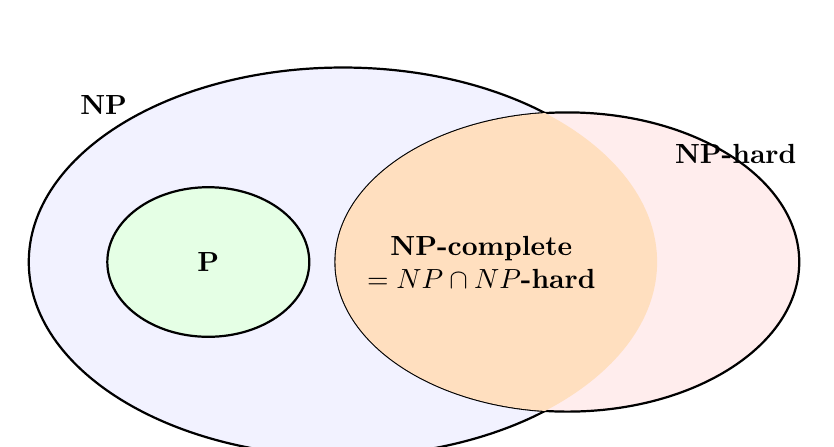
\begin{tikzpicture}[scale=0.95]
  \draw[thick,fill=blue!5] (0,0) ellipse (4.2 and 2.6);
  \node[font=\bfseries] at (-3.2,2.1) {NP};

  \draw[thick,fill=green!10] (-1.8,0) ellipse (1.35 and 1.0);
  \node[font=\bfseries] at (-1.8,0) {P};

  \draw[thick,fill=red!7] (3.0,0) ellipse (3.1 and 2.0);
  \node[font=\bfseries] at (5.25,1.45) {NP-hard};

  \begin{scope}
    \clip (0,0) ellipse (4.2 and 2.6);
    \fill[orange!25] (3.0,0) ellipse (3.1 and 2.0);
  \end{scope}
  \node[font=\bfseries,align=center] at (1.85,0) {NP-complete\\$=NP\cap NP$-hard};
\end{tikzpicture}
\end{center}

\textbf{Definitions and relationships:}
\begin{itemize}[leftmargin=1.5em]
\item \(P\): decision problems solvable in polynomial time by a deterministic algorithm.
\item \(NP\): decision problems whose YES certificates can be verified in polynomial time.
\item \(NP\)-hard: a problem \(H\) is NP-hard if every problem in NP can be polynomial-time reduced to \(H\). An NP-hard problem need not itself belong to NP.
\item \(NP\)-complete: problems that are both in NP and NP-hard:
\[
\boxed{NP\text{-complete}=NP\cap NP\text{-hard}.}
\]
\end{itemize}
Also,
\[
\boxed{P\subseteq NP}.
\]
Whether \(P=NP\) is unknown; the usual diagram draws \(P\) as a proper subset only to illustrate the widely believed case \(P\ne NP\).
\end{qaanswer}

\begin{qaquestion}[Question 5(b) - 8 marks]
Prove that the following feature-selection problem is NP-complete.

You are given a set of features and a collection of labeled examples. Each example is described by the features present in it and has binary label 0 or 1. Two examples are \textbf{conflicting} if they have different labels. A selected feature set is \textbf{consistent} if every conflicting pair can be distinguished using at least one selected feature. Given a positive integer \(k\), determine whether there exists a subset of at most \(k\) features that distinguishes all conflicting pairs.
\end{qaquestion}

\begin{qaanswer}[Answer 5(b)]
We prove NP-completeness by reduction from \textbf{SET COVER}.

\textbf{1. The problem is in NP.}
A certificate is a set \(F'\) of at most \(k\) selected features. For every pair of examples with different labels, check whether at least one selected feature has different values on the two examples. This takes polynomial time. Hence the problem is in NP.

\textbf{2. SET COVER \(\le_p\) Feature Selection.}
Take an instance of SET COVER:
\[
U=\{u_1,\ldots,u_m\},\qquad
\mathcal S=\{S_1,\ldots,S_n\},\qquad k.
\]
Create one feature \(f_j\) for each set \(S_j\).

Create one special example \(x_0\) with label 0 and all feature values 0. For each universe element \(u_i\), create an example \(x_i\) with label 1, defined by
\[
x_i[f_j]=
\begin{cases}
1,&u_i\in S_j,\\
0,&u_i\notin S_j.
\end{cases}
\]
The only relevant conflicting pairs are \((x_0,x_i)\), since all \(x_i\)'s have the same label 1.

A selected feature \(f_j\) distinguishes \(x_0\) from \(x_i\) exactly when
\[
u_i\in S_j.
\]
Therefore a set of at most \(k\) features distinguishes every conflicting pair iff the corresponding \(k\) sets cover every element of \(U\).

The construction is polynomial. Thus SET COVER reduces to the feature-selection problem. Since SET COVER is NP-complete, the feature-selection problem is NP-hard; combined with membership in NP,
\[
\boxed{\text{Feature Selection is NP-complete}.}
\]
\end{qaanswer}

% ===================== Q6 =====================
\begin{qaquestion}[Question 6(a) - 6 marks]
Given a unique character set of size 100 and a maximum pattern length of 7, determine the minimum number of bits required in an integer to design the Rabin-Karp algorithm with linear runtime complexity.
\end{qaquestion}

\begin{qaanswer}[Answer 6(a)]
To eliminate hash collisions completely, encode a pattern of at most 7 characters as an exact base-100 integer.

The number of possible length-7 strings is
\[
100^7=10^{14}.
\]
So we need enough bits to represent values up to \(100^7-1\):
\[
b=\left\lceil\log_2(100^7)\right\rceil
=\left\lceil7\log_2 100\right\rceil.
\]
Since
\[
7\log_2 100\approx46.506,
\]
we get
\[
\boxed{b=47\text{ bits}}.
\]
With exact rolling fingerprints there are no spurious hash matches, so the scan remains linear in the text length after preprocessing.
\end{qaanswer}

\begin{qaquestion}[Question 6(b) - 4 marks]
Given text
\[
T=\texttt{ABABABABC}
\]
and pattern
\[
P=\texttt{ABABC},
\]
find all occurrences of \(P\) in \(T\) using Rabin-Karp. Use
\[
h(S)=\left(\sum_{k=0}^{m-1}\operatorname{value}(s_k)d^{m-1-k}\right)\bmod q,
\]
with \(d=4\), \(q=13\), and character values \(A=0,B=1,C=2\).
\end{qaquestion}

\begin{qaanswer}[Answer 6(b)]
Pattern length is \(m=5\).

Pattern hash:
\[
\begin{aligned}
h(\texttt{ABABC})
&=(0\cdot4^4+1\cdot4^3+0\cdot4^2+1\cdot4+2)\bmod13\\
&=(64+4+2)\bmod13\\
&=70\bmod13=\boxed{5}.
\end{aligned}
\]

The five length-5 windows of \(T\) are:

\begin{center}
\begin{tabular}{c c c c}
\toprule
Shift (0-based) & Window & Hash mod 13 & Match?\\
\midrule
0 & \texttt{ABABA} & 3 & No\\
1 & \texttt{BABAB} & 0 & No\\
2 & \texttt{ABABA} & 3 & No\\
3 & \texttt{BABAB} & 0 & No\\
4 & \texttt{ABABC} & 5 & Yes\\
\bottomrule
\end{tabular}
\end{center}

Only the window at shift 4 has the same hash; direct character verification confirms the match. Therefore
\[
\boxed{P\text{ occurs at 0-based position }4}
\]
or at 1-based position
\[
\boxed{5}.
\]

The rolling update can use
\[
h_0=d^{m-1}\bmod q=4^4\bmod13=9,
\]
\[
t_{s+1}=\bigl(d(t_s-\operatorname{value}(T[s])h_0)+\operatorname{value}(T[s+m])\bigr)\bmod q.
\]
\end{qaanswer}

\begin{qaquestion}[Question 6(c) - 4 marks]
Draw the suffix tree for the string \(\texttt{ABANANA}\).
\end{qaquestion}

\begin{qaanswer}[Answer 6(c)]
Append a unique terminal marker:
\[
X=\texttt{ABANANA\$}.
\]
The suffixes are indexed 0 through 7.

\begin{center}
\resizebox{0.92\textwidth}{!}{%
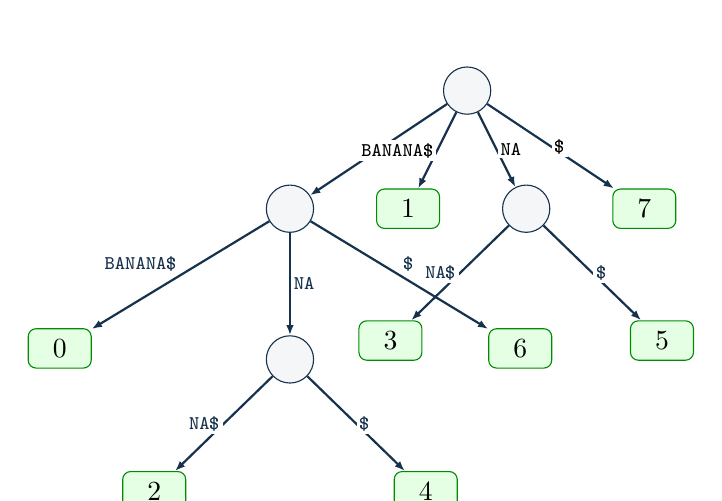
\begin{tikzpicture}[
  level distance=15mm,
  internal/.style={draw=deepnavy,fill=softgray,circle,minimum size=6mm,inner sep=1pt},
  leaf/.style={draw=green!55!black,fill=green!10,rounded corners=1mm,minimum width=8mm,minimum height=5mm},
  edge from parent/.style={draw=deepnavy,thick,-{Latex[length=1.3mm]}},
  lab/.style={midway,fill=white,inner sep=1pt,font=\scriptsize}
]
\node[internal] (r) {}
  child { node[internal] (A) {}
    edge from parent node[lab,left] {\texttt{A}}
  }
  child { node[leaf] {1}
    edge from parent node[lab,left] {\texttt{BANANA\$}}
  }
  child { node[internal] (N) {}
    edge from parent node[lab,right] {\texttt{NA}}
  }
  child { node[leaf] {7}
    edge from parent node[lab,right] {\texttt{\$}}
  };

\node[leaf] (l0) [below left=13mm and 23mm of A] {0};
\node[internal] (ANA) [below=13mm of A] {};
\node[leaf] (l6) [below right=13mm and 23mm of A] {6};
\draw[deepnavy,thick,-{Latex[length=1.3mm]}] (A)--node[lab,above left]{\texttt{BANANA\$}}(l0);
\draw[deepnavy,thick,-{Latex[length=1.3mm]}] (A)--node[lab,right]{\texttt{NA}}(ANA);
\draw[deepnavy,thick,-{Latex[length=1.3mm]}] (A)--node[lab,above right]{\texttt{\$}}(l6);

\node[leaf] (l2) [below left=12mm and 11mm of ANA] {2};
\node[leaf] (l4) [below right=12mm and 11mm of ANA] {4};
\draw[deepnavy,thick,-{Latex[length=1.3mm]}] (ANA)--node[lab,left]{\texttt{NA\$}}(l2);
\draw[deepnavy,thick,-{Latex[length=1.3mm]}] (ANA)--node[lab,right]{\texttt{\$}}(l4);

\node[leaf] (l3) [below left=12mm and 11mm of N] {3};
\node[leaf] (l5) [below right=12mm and 11mm of N] {5};
\draw[deepnavy,thick,-{Latex[length=1.3mm]}] (N)--node[lab,left]{\texttt{NA\$}}(l3);
\draw[deepnavy,thick,-{Latex[length=1.3mm]}] (N)--node[lab,right]{\texttt{\$}}(l5);
\end{tikzpicture}}
\end{center}

The root-to-leaf strings are exactly the suffixes:
\[
\begin{array}{c|l@{\qquad}c|l}
0&\texttt{ABANANA\$}&4&\texttt{ANA\$}\\
1&\texttt{BANANA\$}&5&\texttt{NA\$}\\
2&\texttt{ANANA\$}&6&\texttt{A\$}\\
3&\texttt{NANA\$}&7&\texttt{\$}
\end{array}
\]
\end{qaanswer}

% ===================== Q7 =====================
\begin{qaquestion}[Question 7(a) - 4 marks]
The ski-rental problem is defined as follows. You are going skiing for an unknown number of days. Renting skis costs 500 Taka per day and buying skis costs 1500 Taka. Every day you must decide whether to continue renting for one more day or buy a pair of skis.

Mention the features of an online algorithm. Define the competitive ratio using a strategy for this ski-rental problem.
\end{qaquestion}

\begin{qaanswer}[Answer 7(a)]
\textbf{Features of an online algorithm:}
\begin{itemize}[leftmargin=1.5em]
\item input arrives over time, one request/event at a time;
\item the algorithm must decide using only the information seen so far;
\item future requests are unknown;
\item decisions are normally irrevocable or costly to undo;
\item performance is measured against an optimal offline algorithm that knows the entire future.
\end{itemize}

For a minimization problem, \(A\) is \(c\)-competitive if there is a constant \(\beta\) such that
\[
A(\sigma)\le c\,\OPT(\sigma)+\beta
\]
for every request sequence \(\sigma\).

\textbf{Ski strategy.} Since
\[
\frac{1500}{500}=3,
\]
rent for the first two days; if skiing continues to day 3, buy at the beginning of day 3.

For \(N\) skiing days,
\[
A(N)=
\begin{cases}
500,&N=1,\\
1000,&N=2,\\
2500,&N\ge3,
\end{cases}
\]
while
\[
\OPT(N)=\min(500N,1500).
\]
Hence the worst ratio is
\[
\max_N\frac{A(N)}{\OPT(N)}
=\frac{2500}{1500}
=\boxed{\frac53}.
\]
So this threshold strategy is \(5/3\)-competitive for these particular costs.
\end{qaanswer}

\begin{qaquestion}[Question 7(b) - 10 marks]
Consider the online linear-list search problem. The cost of accessing an item is proportional to its distance from the head of a linked list, and a request sequence of accesses is given. The objective is to reorder the list so that total access cost is minimized.

\begin{enumerate}[label=(\roman*),leftmargin=2em]
\item (4 marks) Consider a case in which the accessed item is moved two positions forward, and the request sequence is only for the same item of the list. Calculate the competitive ratio.
\item (6 marks) Prove that no algorithm has a competitive ratio better than 2 for the linear-list search problem.
\end{enumerate}
\end{qaquestion}

\begin{qaanswer}[Answer 7(b)]
\textbf{(i) Move-ahead-two strategy.}

The scan is slightly unclear after the words ``the item of the list.'' We use the natural standard interpretation: the request sequence repeatedly requests one fixed item, and for the worst case that item starts at the last position \(n\).

The online strategy moves the accessed item forward by only two positions after each access. Thus its access positions are
\[
n,n-2,n-4,\ldots
\]
until it reaches the front.

If \(n=2r\), consider the first \(r\) requests. The online cost is
\[
A=r(r+1)
\]
because
\[
2r+(2r-2)+\cdots+2=r(r+1).
\]
The offline optimum pays \(2r\) on the first request, moves the item to the front, and then pays 1 thereafter:
\[
\OPT=2r+(r-1)=3r-1.
\]
Therefore
\[
\frac{A}{\OPT}
=\frac{r(r+1)}{3r-1}
=\Theta(r)=\Theta(n).
\]
So the move-ahead-two rule is \textbf{not constant-competitive}; its competitive ratio can grow linearly with the list size:
\[
\boxed{\text{competitive ratio}=\Theta(n).}
\]

\medskip
\textbf{(ii) Lower bound of 2 for deterministic online list search.}

Consider any deterministic online algorithm \(A\). An adaptive adversary always requests the item currently at the last position of \(A\)'s list. Therefore \(A\) pays \(n\) for every request. For \(m\) requests,
\[
A(\sigma)=mn.
\]

Now compare with a fixed offline ordering. If a list ordering is chosen uniformly at random, every requested item has expected position
\[
\frac{n+1}{2}.
\]
Hence the expected total access cost of that random fixed ordering is
\[
\frac{m(n+1)}{2}.
\]
By the averaging principle, at least one fixed ordering has cost no larger than this. Therefore the offline optimum satisfies, up to an initial rearrangement additive constant,
\[
\OPT(\sigma)\le\frac{m(n+1)}{2}+O(n^2).
\]
For long sequences,
\[
\frac{A(\sigma)}{\OPT(\sigma)}
\ge
\frac{mn}{m(n+1)/2+O(n^2)}
\longrightarrow
\frac{2n}{n+1}.
\]
As \(n\to\infty\),
\[
\frac{2n}{n+1}\to2.
\]
Thus no deterministic online algorithm can have competitive ratio strictly below 2 in the asymptotic worst case:
\[
\boxed{c\ge2.}
\]
\end{qaanswer}

% ===================== REVISION =====================
\clearpage
\begin{center}
{\LARGE\bfseries\color{primary} Last-Minute Revision Sheet}
\end{center}

\begin{pointbox}[Hashing]
\begin{itemize}[leftmargin=1.5em]
\item Primary clustering: long contiguous occupied runs, especially in linear probing.
\item Quadratic: \(h(k,i)=(h'(k)+C_1i+C_2i^2)\bmod m\).
\item Double hash: \(h(k,i)=(h_1(k)+i h_2(k))\bmod m\).
\item Uniform hashing unsuccessful search: \(E[X]\le1/(1-\alpha)\).
\end{itemize}
\end{pointbox}

\begin{pointbox}[Geometry and Backtracking]
\begin{itemize}[leftmargin=1.5em]
\item Adding a point to a set cannot shrink its convex hull: \(A\le B\).
\item Ellipse boundary intersection: parameterize one ellipse and solve \(F(t)=0\).
\item Sudoku: choose empty cell, try safe digits, recurse, undo on failure.
\item Branch-and-bound: compute a safe upper bound; if \(UB\le k\), prune.
\end{itemize}
\end{pointbox}

\begin{pointbox}[String Matching]
\begin{itemize}[leftmargin=1.5em]
\item KMP pattern \texttt{AABA}: \(\pi=[0,1,0,1]\); matches in the given text at 0-based shifts \(0,9,12\).
\item 2-D KMP: horizontal row matching + vertical KMP on row IDs.
\item Rabin-Karp exact base-100 code for length 7 needs 47 bits.
\item \texttt{ABABC} occurs once in \texttt{ABABABABC}, at 0-based shift 4.
\end{itemize}
\end{pointbox}

\begin{pointbox}[Complexity and Online Algorithms]
\begin{itemize}[leftmargin=1.5em]
\item \(P\subseteq NP\), \(NP\)-complete \(=NP\cap NP\)-hard.
\item Feature selection is NP-complete via SET COVER.
\item Ski rental with rent 500, buy 1500: buy on day 3 after two rentals; ratio \(5/3\).
\item Deterministic online list search has lower bound 2.
\end{itemize}
\end{pointbox}

\end{document}
